\section{INTRODUCTION}
\label{sec:intro}
The main purpose of indoor scene layout estimation is to extract semantic boundaries among walls, ceiling and floor, and to obtain different planes which provide strong spacial expression of the scene, for cluttered indoor scenes from a single RGB image, as shown in Fig. \ref{fig:definition}. 


\begin{figure}[!ht]
	\centering
	\textsc{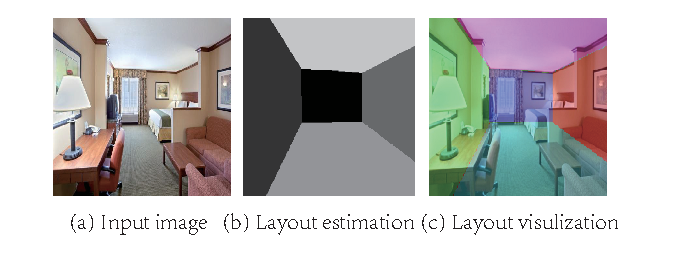
\includegraphics[width=3.5in]{figure/definition.eps}}
	\caption{Examples of indoor scene images. (a) Input images. (b) Layout estimation with semantic labels. (c) Layout visulization superimposed on the input image.}
	\label{fig:definition}
\end{figure}


Layout estimation is a fundamental and indispensable problem for indoor scene understanding, and it plays a critical role in a diverse range of hot applications, such as scene reconstruction, robot navigation, virtual reality, and so on. Moreover, on the Large-scale Scene Understanding Challenge(LSUN), indoor scene layout estimation has become one of the popular tasks towards scene-centric challenges. However, the most important clues such as room corners and layout boundaries are often occluded by a large amount of clutter occuring everywhere in daily life(see Fig.\ref{fig:pipeline} (a)), which make the layout task tough to estimate. Moreover,  illumination variations existed in indoor scene(see Fig.\ref{fig:pipeline} (b-c)), may increase the difficulty of visual understanding. Last but not the least, the views of indoor scene images are in a wide range(see Fig.\ref{fig:pipeline} (d-f)), and such factor can  cause appearance diversity for an indoor scene image.


\begin{figure}[!ht]
	\centering
	\textsc{\includegraphics[width=3.5in]{figure/case.eps}}
	\caption{Examples of indoor scene images. (a) Much clutter. (b) Too bright. (c) Too dark. (d-f) Different views.}
	\label{fig:case}
\end{figure}

\cxj{Related work: from estimation using vanishing points/low-level features, then two-step (FCN+post-processing), to end-to-end network. }
%%
In recent decades, many researchers have made massive attempts to estimate spacial layout from a single image automatically. One popular framework using a 3D cuboid to approximately express indoor scene layout was introduced by \cite{hedau2009recovering} in 2009. The author generated several layout candidates by using vanish point detection. Then it gathered mid-level features like the line membership features and the geometric context features for each candidate and ranked them by using a structured SVM. Unfortunately, the process of layout candidiate generation is highly sensitive and fragile towards a large amount of clutter. Based on this milestone work, several strategies focused on layout hypothesis generation and ranking were considered. Wang et al.\cite{wang2013discriminative} introduced latent variables to model indoor clttuer. Moreover, in \cite{schwing2012efficient}\cite{schwing2013box}, Schwing et al. modeled cllutterd indoor scenes with higher-order potentials and jointly generated layout and objects with box shapes. Some researchers introduced low-level information as geometric restrictions as supplementary in indoor scene problem. Lee et al.\cite{lee2009geometric}. proposed several physically valid structure hypotheses by geometric reasoning and verified to find the best fitting model to line segments. Ramalingam et al.\cite{ramalingam2013manhattan} employed Manhattan Junction grouping to select best layout. As mentioned above, traditional methods need to design image features manually, which greatly increase the complexity and are weekly capable of adapting to dealing with all complex indoor scenes. Besides, there exists a large time consuming for layout candidate generation, which is stongly against our intention to rely on computers to understand the room layout as fastly as possible.

Since the development of the 3D-data capture devices like kinects and RGBD depth cameras, more and more 3D-based methods towards indoor scene field have been studied. Moreover, some researches using 3D-based methods for indoor layout estimation have been studied. Geiger et al.\cite{geiger2015joint} proposed a high-order graphical model and jointly reasoned about the layout, objects and superpixels from RGBD image. Ren et al.\cite{ren2016three} proposed a cloud of oriented gradient descriptor and “Manhattan voxel” that links the 2D appearance and 3D pose of object categories to better capture the 3D room layout geometry and object detection. Guo et al.\cite{guo2015predicting} interpreted layout and 3D model jointly from a RGBD image by aligning to 3D model dataset. 3D information provide additional geometric cues based on planes and objects, which merge big planes and obejects together and weaken the effects of light and complex textures, and thus lead to robust semantic understanding. With 3D-based methods, not only can layout estimation work turn out to be more robust, but also more problems we can solve even 3D modeling  problem for whole indoor scenes.  

Recently, the deep learning methods and convolution neural network(CNN) have achived impressive progresses in various computer vision tasks, such as semantic segmentation \cite{long2015fully}\cite{chen2016deeplab}, object detection \cite{girshick2015fast}\cite{ren2015faster}, scene understanding \cite{gupta2015indoor}\cite{badrinarayanan2017segnet}, and so on. Towards layout estimation problem, several researchers have achieved to adopt deep learning methods to solve it. Mallya et al.\cite{mallya2015learning}, presented a Fully Convolutional Networks (FCNs)\cite{long2015fully} framwork for learning informative edge maps from a single image, which provided as a new information to sample vanishing lines for layout candidates generation and ranking. This work is the first to train CNN to produce robust features used to replace hand-crafted features towards layout estimation problem. However, in the framwork of layout candidates generation and ranking, their algorithm still remained time-consuming. Dasgupta et al.\cite{dasgupta2016delay} used the FCN to learn semantic surface labels including left wall, front wall, right wall, ceiling, and ground. Initial layout generation and optimization were all based on suface belif labels. Unfortunately, Their algorithm relies entirely on FCN's precision for semantic surface labels. In other words, if FCN result gains two much error, we may get totally wrong prediction. Moreover, optimization procedure does not utilize any restrictions based on edge information, just taking random combinations of edges instead, which is geometric inconformity compared with RGB images. Ren et al.\cite{ren2016coarse} adopted a multi-task fully convolutional neural network (MFCN) to jointly predict the room edges and semantic labels. Then a coarse-to-fine method was adopted which enforced several constraints such as layout contour straightness, surface smoothness and geometric constraints to generate fine layout from coarse prediction of room edges. They have considerd geometric constraints to predict high quality estimation results. They need complex geometric computation and rules to generate useful critical lines, however, such low-level features are exactly what we avoid to extract. Zhang et al.\cite{zhang2016learning} used another deconvolution network which has multi-layer deconvolution and a receptive field as large as the entire image compared to FCN. As the result, they can obtain highly reliable edge maps. Then they follow the framework of layout candidates generation using vanish line samplling with an adaptive line sample strategy for robustness and time reduction. A measurement of similarity is proposed between edge map and layout candidates for ranking. Unexpectedly, their results are less precise compared with \cite{dasgupta2016delay}\cite{ren2016coarse}. One explanation may be that the latter two optimization strategies are more effective compared to vanish line sampling.

\cxj{compared to \cite{ren2016coarse}, what is our advantage? They apply geometric constraints as an optimization problem. \cite{dasgupta2016delay} also apply a post-processing step to enforce geometric constraints. One big disadvantage of the post-processing is that it takes seconds to optimize the layout. \cite{dasgupta2016delay} requires 30 seconds for the layout optimization.}\\
\drf{compared to \cite{ren2016coarse}, we have better performance on layout estimation before optimization. ie. the output of our FCN-MC are more reliable because we apply additional information(depth and normals). We use the same post-processing step in \cite{dasgupta2016delay}, so we have the same problem, or maybe worse.}

\cxj{\cite{LeeRoomNet17} presents an end-to-end trainable network that predicts the layout corners and room type A RNNN framework is employed to refine the layout. Different from previous pixel-based representation of the layout, they use a keypoint-based representation.  }

In this work, our algorithm is based on framework of \cite{dasgupta2016delay}, which does not need to extract low features of lines and vanish points from a single RGB image. To enhance the existed FCN's ability, we use networks to estimate depth and normal information from one single RGB image. Then depth and normal information serves as geomtric embedded into FCN networks to jointly generate high quality suface maps and edge maps. Based on\cite{dasgupta2016delay} optimization framwork, we introduce more geometric constraints from predicted edge maps to optimize surface labels to generate high quality layout estimation. Experimental results demonstrate that our method is robust and effective for layout estimation even facing a high clutter on two popular room layout benchmark datasets.
 
 




	
	

